\documentclass{standalone}
\usepackage{tikz}
\usetikzlibrary{positioning}
\usetikzlibrary{decorations.pathmorphing}

\tikzset{snake it/.style={decorate, decoration={snake, segment length=1.5mm, amplitude=0.5mm}}}
\tikzset{
    position/.style args={#1:#2 from #3}{
        at=(#3.#1), anchor=#1+180, shift=(#1:#2)
    }
}

\begin{document}
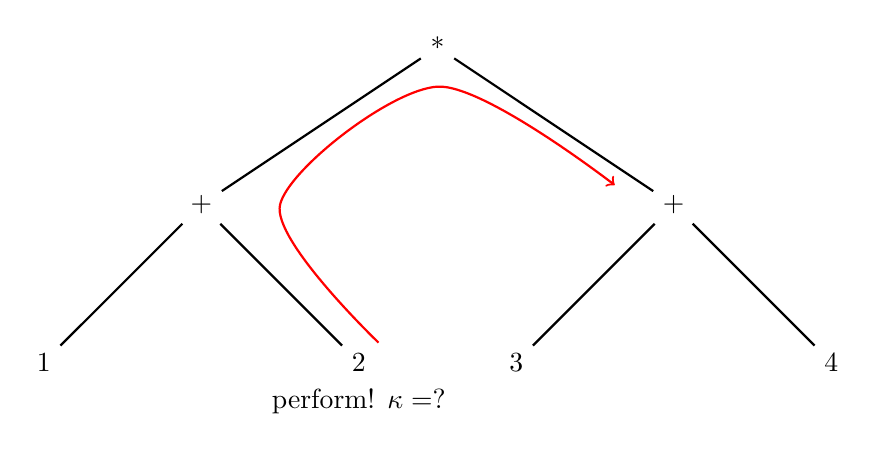
\begin{tikzpicture}
    \node (ROOT) at (5,0) {*};
    \node (LPLUS) at (2,-2) {+};
    \node (RPLUS) at (8,-2) {+};
    
    \node (ONE) at (0,-4) {1};
    \node (TWO) at (4, -4) {2}; \node (CONT) at (4, -4.5) {perform! $\kappa = ?$};
    \node (THREE) at (6, -4) {3};
    \node (FOUR) at (10, -4) {4};

    \draw[thick] (ONE) -- (LPLUS);
    \draw[thick] (TWO) -- (LPLUS);

    \draw[thick] (THREE) -- (RPLUS);
    \draw[thick] (FOUR) -- (RPLUS);

    \draw[thick] (LPLUS) -- (ROOT);
    \draw[thick] (RPLUS) -- (ROOT);

    \draw[->, red, thick] plot [smooth] coordinates {(4.25,-3.75) (3,-2) (5,-0.5) (7.25,-1.75)};
    
    % \draw[help lines] (0,0) grid (10,-10);
\end{tikzpicture}
\end{document}